\chapter{网络}

\section{因特网}

\subsection{因特网(Internet)}

因特网是一个世界范围的计算机网络,它互联了遍及全世界数十亿的计算设备,所有这些设备都称为主机(host)或端系统(end system)。端系统通过通信链路(communication link)和分组交换机(packet switch)连接到一起,不同的链路能够以不同的速率传输数据,链路的传输速率(transmission rate)使用比特/秒(bps, bit/s)来度量。端系统通过因特网服务提供商(ISP, Internet Service Provider)接入因特网。\\

当一台端系统向另一台端系统发送数据时,发送端将数据分组,发送到目的端系统,在那里进行组装。一个分组所经历的一系列通信链路和分组交换机称为路径(route / path)。分组交换类似于现实中的货物运输,在出发地将货物分开并装上多辆卡车,每辆卡车独立通过公路运输,最后在目的地卸货并重新组装。

\begin{figure}[H]
    \centering
    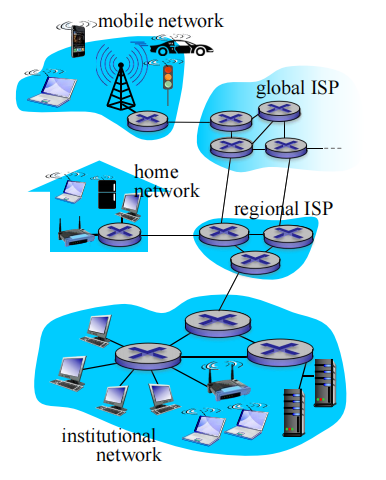
\includegraphics[scale=0.8]{img/C1/1-1/1.png}
    \caption{计算机网络}
\end{figure}

\vspace{0.5cm}

\subsection{分布式应用程序(Distributed Application)}

分布式应用程序涉及多个相互交换数据的端系统,例如即时通信、实时道路信息、视频会议、多人游戏等。分布式应用程序的核心问题在于一个端系统上的应用程序如何能够向运行在另一个端系统上的应用程序发送数据。\\

套接字接口(socket interface)规定了运行在一个端系统上的程序向运行在另一个端系统上的特定程序交付数据的方式。例如Alice要给Bob寄一封信,当然Alice不能只是写完这封信就把它丢出窗外。Alice需要把信放入信封,在信封上根据指定格式写上收信人的全名、地址和邮政编码,信封上贴上邮票,再将信封投入信箱中。Alice想要寄信就必须要遵守邮政服务制定的这一套规则。因此,发送数据的程序也必须遵守socket接口,才能向接收数据的程序发送数据。\\

\subsection{协议(Protocol)}

在两个人或两台设备之间进行通信时需要遵守一些协议,协议就是用于管理通信的一组规则。传输控制协议TCP(Transmission Control Protocol)和网际协议IP(Internet Protocol)是因特网中两个最为重要的协议,因特网的主要协议统称为TCP/IP。\\

因特网标准(Internet standard)是经过充分测试的规约,只要是与因特网打交道,就会用到它们,并要服从于它们。因特网标准由IETF(Internet Engineering Task Force)研发,IETF的标准文档称为RFC (Request For Comment),目的是解决因特网先驱者们面临的网络和协议问题。它们定义了TCP、IP、HTTP、SMTP等协议,目前已经有将近7000个RFC。\\

人类无时无刻都在执行协议,人类用约定好的交互方式互相交流。但是如果两人的交谈都不在同一频道上,那就不能好好沟通了。\\

\begin{figure}[H]
    \centering
    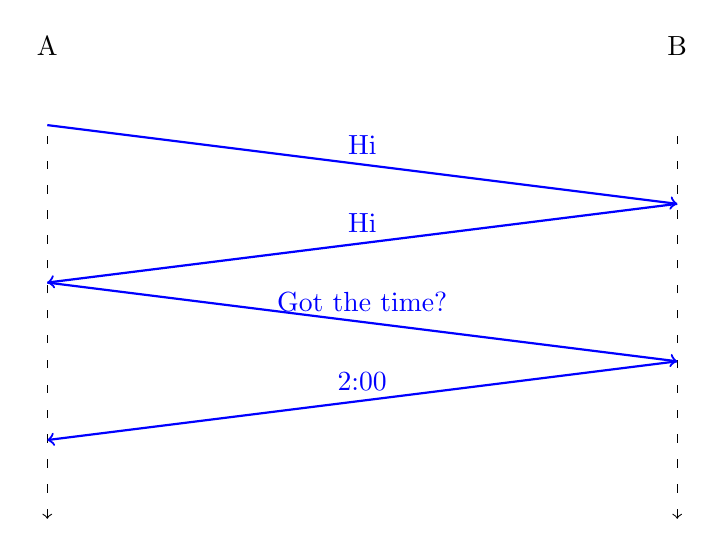
\begin{tikzpicture}
        \node at (0,6) {A};
        \node at (8,6) {B};

        \draw[loosely dashed, <-] (0,0) -- (0,5);
        \draw[loosely dashed, <-] (8,0) -- (8,5);

        \draw[blue, ->, thick] (0,5) -- (4,4.5) node[above]{Hi} -- (8,4);
        \draw[blue, ->, thick] (8,4) -- (4,3.5) node[above]{Hi} -- (0,3);
        \draw[blue, ->, thick] (0,3) -- (4,2.5) node[above]{Got the time?} -- (8,2);
        \draw[blue, ->, thick] (8,2) -- (4,1.5) node[above]{2:00} -- (0,1);
    \end{tikzpicture}
    \caption{人类协议}
\end{figure}

在因特网中,涉及两个或多个远程通信实体的所有活动都受协议的制约。例如在浏览器中输入URL(Uniform Resource Locator)向一个Web服务器发出请求,首先你的计算机将向该Web服务器发送一条连接请求报文,并等待回答。Web服务器接收到连接请求报文,并返回一条连接响应报文。在得知请求正常后,计算机会发送一条要获取的网页名字的报文,最后Web服务器向计算机返回该网页。\\

\begin{figure}[H]
    \centering
    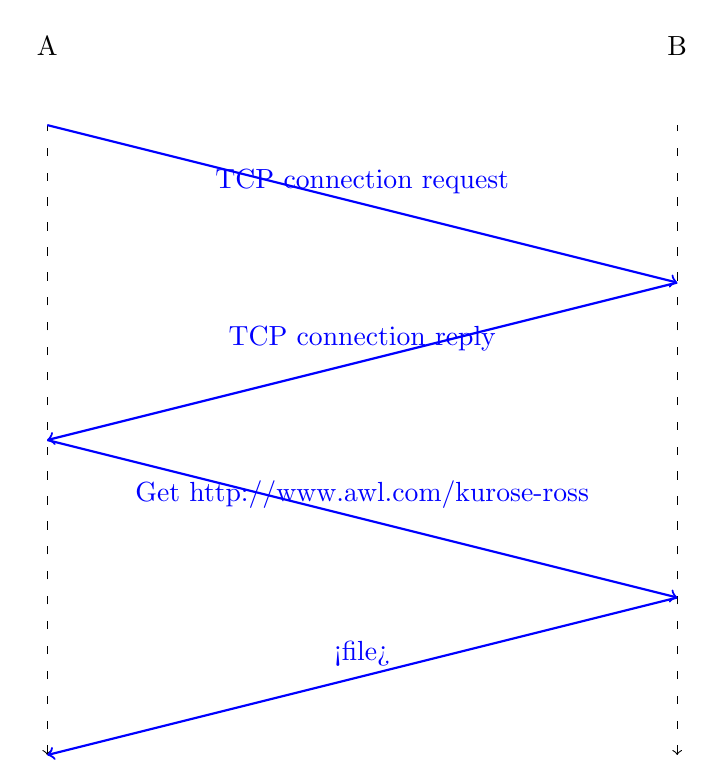
\begin{tikzpicture}
        \node at (0,9) {A};
        \node at (8,9) {B};

        \draw[loosely dashed, <-] (0,0) -- (0,8);
        \draw[loosely dashed, <-] (8,0) -- (8,8);

        \draw[blue, ->, thick] (0,8) -- (4,7) node[above]{TCP connection request} -- (8,6);
        \draw[blue, ->, thick] (8,6) -- (4,5) node[above]{TCP connection reply} -- (0,4);
        \draw[blue, ->, thick] (0,4) -- (4,3) node[above]{Get http://www.awl.com/kurose-ross} -- (8,2);
        \draw[blue, ->, thick] (8,2) -- (4,1) node[above]{<file>} -- (0,0);
    \end{tikzpicture}
    \caption{网络协议}
\end{figure}

\newpage

\section{分组交换}

\subsection{存储转发传输(Store-and-Forward Transmission)}

在网络应用中,端系统彼此交换报文(message),报文能够包含任何数据。报文从源端系统发送到目的端系统的过程中,长报文会被划分为较小的数据块,称为分组(packet),每个分组都通过通信链路和分组交换机传送。如果源端系统发送一个$ L $ bits分组,链路的传输速率为$ R $ bits/sec,则传输该分组的时间为$ L \over R $秒。\\

多数分组交换机在链路的输入端使用存储转发传输机制,存储转发传输是指在交换机能够开始向输出链路传输该分组的第一个bit之前,必须接收到整个分组。\\

\begin{figure}[H]
    \centering
    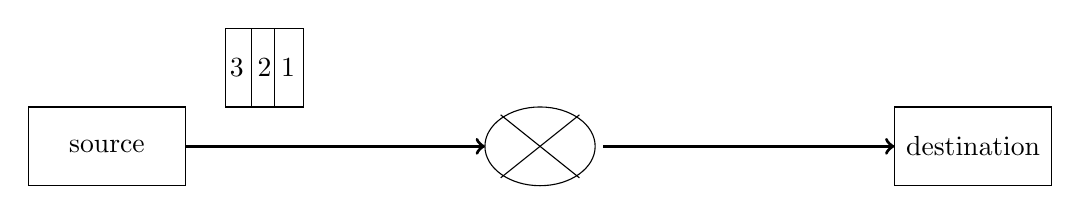
\begin{tikzpicture}
        \draw (0,0) rectangle (2,1);
        \node at (1,0.5) {source};
        \draw (11,0) rectangle (13,1);
        \node at (12,0.5) {destination};
        \draw (6.5,0.5) ellipse (0.7 and 0.5);
        \draw[-] (6,0.9) -- (7,0.1);
        \draw[-] (7,0.9) -- (6,0.1);

        \draw[->, very thick] (2,0.5) -- (5.8,0.5);
        \draw[->, very thick] (7.3,0.5) -- (11,0.5);

        \draw (2.5,1) rectangle (3.5,2);
        \draw (2.833,1) -- (2.833,2);
        \draw (3.133,1) -- (3.133,2);
        \node at (2.65,1.5) {3};
        \node at (3,1.5) {2};
        \node at (3.3,1.5) {1};
    \end{tikzpicture}
    \caption{存储转发}
\end{figure}

假设忽略传播时延(propagation delay),源端系统在时间0开始传输,路由器在时间$ L \over R $刚好接收到整个分组,之后再向输出链路开始传输,在时间$ 2 {L \over R} $整个分组被目的端系统接收。\\

因此,由$ N $条速率为$ R $的链路组成的路径(在源和目的地之间有$ N - 1 $台路由器)发送一个分组,端到端的时延为

\vspace{-0.5cm}

\begin{align}
    d = N {L \over R}
\end{align}

\vspace{0.5cm}

\subsection{时延}

当从一个节点到后继节点,一个分组在沿途的每个节点都经受了几种不同类型的时延,包括节点处理时延(nodal processing delay)、排队时延(queuing delay)、传输时延(transmission delay)、传播时延(propagation delay)。\\

处理时延包括了检查分组首部和决定分组去向所需要的时间,以及检查差错的时间。\\

分组交换机的每条链路都有一个输出缓存/输出队列(output buffer / output queue)。如果到达的分组需要传输到某条链路,但发现该链路正忙于传输其它分组,该分组必须在输出缓存中等待。因此,除了存储转发时延以外,分组还要承受输出缓存的排队时延。由于缓存空间的大小是有限的,到达的分组可能发现该缓存已被填满,这种情况下将出现丢包(packet loss),到达的分组或已经排队的分组将被丢弃。\\

\begin{figure}[H]
    \centering
    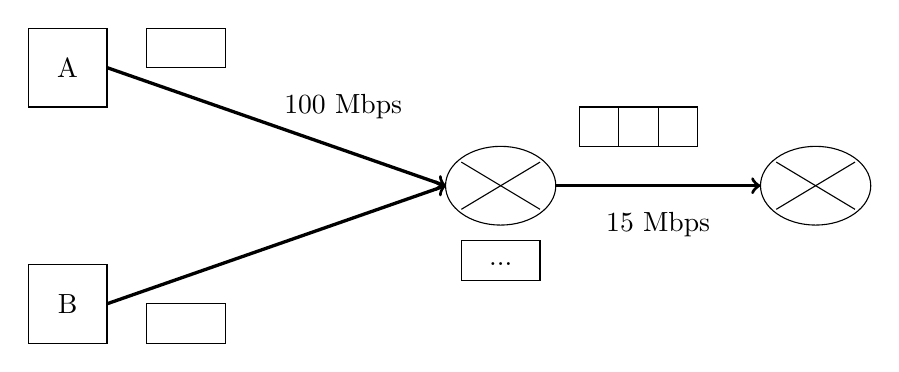
\begin{tikzpicture}
        \draw (0,1) rectangle (1,2);
        \node at (0.5,1.5) {A};
        \draw (0,-2) rectangle (1,-1);
        \node at (0.5,-1.5) {B};

        \draw (6,0) ellipse (0.7 and 0.5);
        \draw[-] (5.5,0.3) -- (6.5,-0.3);
        \draw[-] (5.5,-0.3) -- (6.5,0.3);

        \draw[->, very thick] (1,1.5) -- (5.3,0);
        \draw[->, very thick] (1,-1.5) -- (5.3,0);

        \draw (1.5,1.5) rectangle (2.5,2);
        \draw (1.5,-2) rectangle (2.5,-1.5);
        \node at (4,1) {100 Mbps};

        \draw (10,0) ellipse (0.7 and 0.5);
        \draw[-] (9.5,0.3) -- (10.5,-0.3);
        \draw[-] (9.5,-0.3) -- (10.5,0.3);

        \draw[->, very thick] (6.7,0) -- (9.3,0);

        \draw (7,0.5) rectangle (8.5,1);
        \draw[-] (7.5,0.5) -- (7.5,1);
        \draw[-] (8,0.5) -- (8,1);
        \node at (8,-0.5) {15 Mbps};

        \draw (5.5,-1.2) rectangle (6.5,-0.7);
        \node at (6,-1) {...};
    \end{tikzpicture}
    \caption{排队时延}
\end{figure}

\vspace{0.5cm}

分组通常是以FCFS(First-Come-First-Served)的方式传输,只有当所有以及达到的分组被传输之后,才能传输新到达的分组。传输时延$ L \over R $就是将所有分组推向输出链路所需的时间。\\

传播时延是指从链路的起点到下一个路由器传播所需的时间。\\

假设$ d_{proc} $、$ d_{queue} $、$ d_{trans} $和$ d_{prop} $分别表示处理时延、排队时延、传输时延和传播时延,那么节点总时延为

\vspace{-0.5cm}

\begin{align}
    d_{nodal} = d_{proc} + d_{queue} + d_{trans} + d_{prop}
\end{align}

\begin{figure}[H]
    \centering
    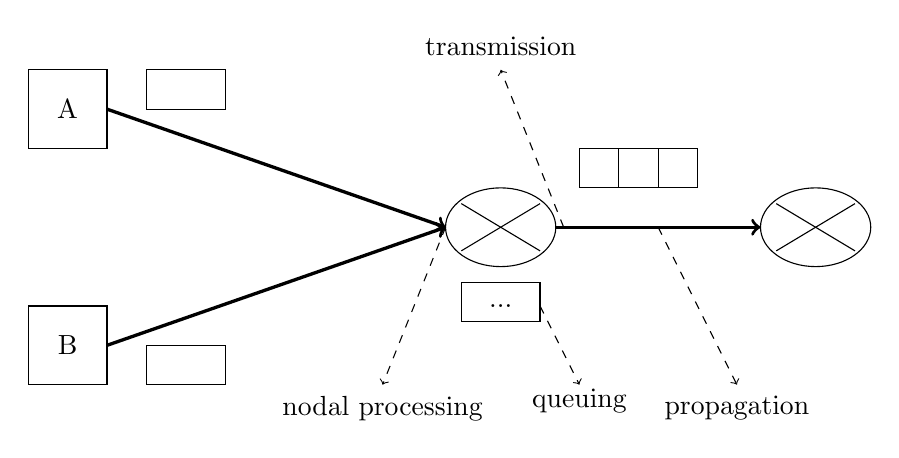
\begin{tikzpicture}
        \draw (0,1) rectangle (1,2);
        \node at (0.5,1.5) {A};
        \draw (0,-2) rectangle (1,-1);
        \node at (0.5,-1.5) {B};

        \draw (6,0) ellipse (0.7 and 0.5);
        \draw[-] (5.5,0.3) -- (6.5,-0.3);
        \draw[-] (5.5,-0.3) -- (6.5,0.3);

        \draw[->, very thick] (1,1.5) -- (5.3,0);
        \draw[->, very thick] (1,-1.5) -- (5.3,0);

        \draw (1.5,1.5) rectangle (2.5,2);
        \draw (1.5,-2) rectangle (2.5,-1.5);

        \draw (10,0) ellipse (0.7 and 0.5);
        \draw[-] (9.5,0.3) -- (10.5,-0.3);
        \draw[-] (9.5,-0.3) -- (10.5,0.3);

        \draw[->, very thick] (6.7,0) -- (9.3,0);

        \draw (7,0.5) rectangle (8.5,1);
        \draw[-] (7.5,0.5) -- (7.5,1);
        \draw[-] (8,0.5) -- (8,1);

        \draw (5.5,-1.2) rectangle (6.5,-0.7);
        \node at (6,-1) {...};
        \draw[dashed, ->] (6.5,-1) -- (7,-2);
        \node at (7,-2.2) {queuing};

        \draw[dashed, ->] (5.3,0) -- (4.5,-2);
        \node at (4.5,-2.3) {nodal processing};

        \draw[dashed, ->] (6.8,0) -- (6,2);
        \node at (6,2.3) {transmission};

        \draw[dashed, ->] (8,0) -- (9,-2);
        \node at (9,-2.3) {propagation};
    \end{tikzpicture}
    \caption{时延}
\end{figure}

\vspace{0.5cm}

\subsection{转发表(Forwarding Table)}

路由器从输入链路获得分组,然后向输出链路发送分组,但是路由器怎样决定应当向哪一条链路发送呢?\\

因特网中每一个端系统都有一个IP地址,源在发送分组时在分组首部包含了目的地的IP地址。当分组达到每一个路由器时,路由器根据转发表,为其查询适当的输出链路。\\

端到端的选路过程类似于现实中的问路,每到一个地点都询问别人路线,逐步找到最终的目的地。在这个类比中,被问路的人就类似于路由器。\\

\subsection{traceroute}

traceroute是诊断网络问题时常用的工具,它可以定位从源主机到目标主机之间经过了哪些路由器,以及到达各个路由器的耗时。当源主机向目标主机发送消息,发现消息无法送达。此时,可能是某个中间节点发生了问题,比如某个路由器因负载过高产生了丢包。通过traceroute可以定位网络包在是在哪个节点丢失的。\\

traceroute将从源发送N个特殊的分组,当第i个路由器收到第i个分组时,该路由器会向源回送一个报文,记录了路由器的名字和地址。traceroute会重复该实验3次。\\

\mybox{traceroute (Linux) / tracert (Windows)}

\begin{lstlisting}
tracert www.github.com
\end{lstlisting}

\begin{tcolorbox}
	\mybox{运行结果}
	\begin{verbatim}
1     2 ms     9 ms     2 ms  HS8145V [192.168.1.1]
2     5 ms    15 ms     5 ms  100.65.0.1
3     5 ms     5 ms     5 ms  124.74.22.41
4    25 ms     6 ms    17 ms  101.95.88.138
5     *        *        *     请求超时。
6     *        *        *     请求超时。
7     *        *        *     请求超时。
8    30 ms    32 ms    35 ms  106.38.244.146
9     *        *        *     请求超时。
10     *        *        *     请求超时。
11     *        *        *     请求超时。
12    30 ms    31 ms    31 ms  220.181.38.251
	\end{verbatim}
\end{tcolorbox}

\newpage